\documentclass{article}

\usepackage[nonanonymous]{neurips_2026}
\usepackage[utf8]{inputenc}
\usepackage[T1]{fontenc}
% Vector typewriter font; the default T1 one is a bitmap font that renders poorly.
\renewcommand{\ttdefault}{lmtt}
\usepackage{hyperref}
\usepackage{url}
\usepackage{booktabs}
\usepackage{tabularx}
\usepackage{array}
\newcolumntype{Y}{>{\raggedright\arraybackslash}X}
\newcolumntype{P}[1]{>{\raggedright\arraybackslash}p{#1}}
\usepackage{graphicx}
\usepackage{amsfonts}
\usepackage{microtype}
\usepackage{xcolor}
\usepackage{enumitem}
\usepackage[strings,nohyphen]{underscore}
\setcitestyle{numbers,square,comma}
\setlist{nosep,leftmargin=*}
\hypersetup{hidelinks}
\renewcommand{\arraystretch}{1.25}

% Red markers for material the group still has to supply. Search for "TODO" before submitting.
\newcommand{\todo}[1]{\textcolor{red}{\textbf{[TODO: #1]}}}
% Code names never break with a hyphen.
\newcommand{\code}[1]{{\ttfamily\small\hyphenchar\font=-1\relax #1}}
% Issue codes inside tables.
\newcommand{\issue}[1]{{\ttfamily\footnotesize\hyphenchar\font=-1\relax #1}}

\makeatletter
\renewcommand{\@noticestring}{COMP7608B Group 52 Final Report}
\makeatother

\title{PaperTrace: A Research Assistant Agent}

\author{
  Group 52\\
  Gong Xiangwei (3036791411) \quad Hou Jiachen (3036808044)\\
  Ning Ziyang (3036790431) \quad Wang Yao (3036806785)
}

\begin{document}

\maketitle
\nolinenumbers

\section{Users, scope and what changed since the proposal}
\label{sec:scope}

\paragraph{Users and needs.}
PaperTrace is for students and researchers who work from a small set of papers they have chosen
themselves: a thesis topic, a related-work section, or a reading group. They ask questions about these
papers, compare them, and check whether the citations in their own drafts say what the cited paper says.
Their main problem is not finding \emph{an} answer but trusting it. A fluent summary is of little use if
the reader still has to open each PDF to find the sentence that supports it.

\paragraph{Core requirements.}
We kept four requirements from the proposal.
(R1) Every factual sentence in an answer either links to a verbatim passage that the agent actually
read, or says that the evidence is missing.
(R2) The user decides which papers and which text may be used, and confirms each task before any
material is sent to a model provider.
(R3) The agent decides what to search and read, within a fixed budget, and stops with a partial or
failed result instead of guessing when the budget, the model or the source text runs out.
(R4) Papers, notes and conversations stay in a local workspace.

\paragraph{Delivered system.}
The submission is a desktop application (Windows and macOS, Tauri + React) with a bundled Python worker
and a Node agent loop. Users create a topic, import PDFs or find papers through OpenAlex, then work in
five views: \emph{Read \& Ask} (cited question answering with a PDF reader), \emph{Compare}, a
per-topic \emph{Wiki}, \emph{Citation check} for their own manuscript PDF, and \emph{Library}.
Figure~\ref{fig:reader} shows Read \& Ask with a full paper open. The submitted source version is
commit \code{f84aee37}.

\begin{figure}[t]
  \centering
  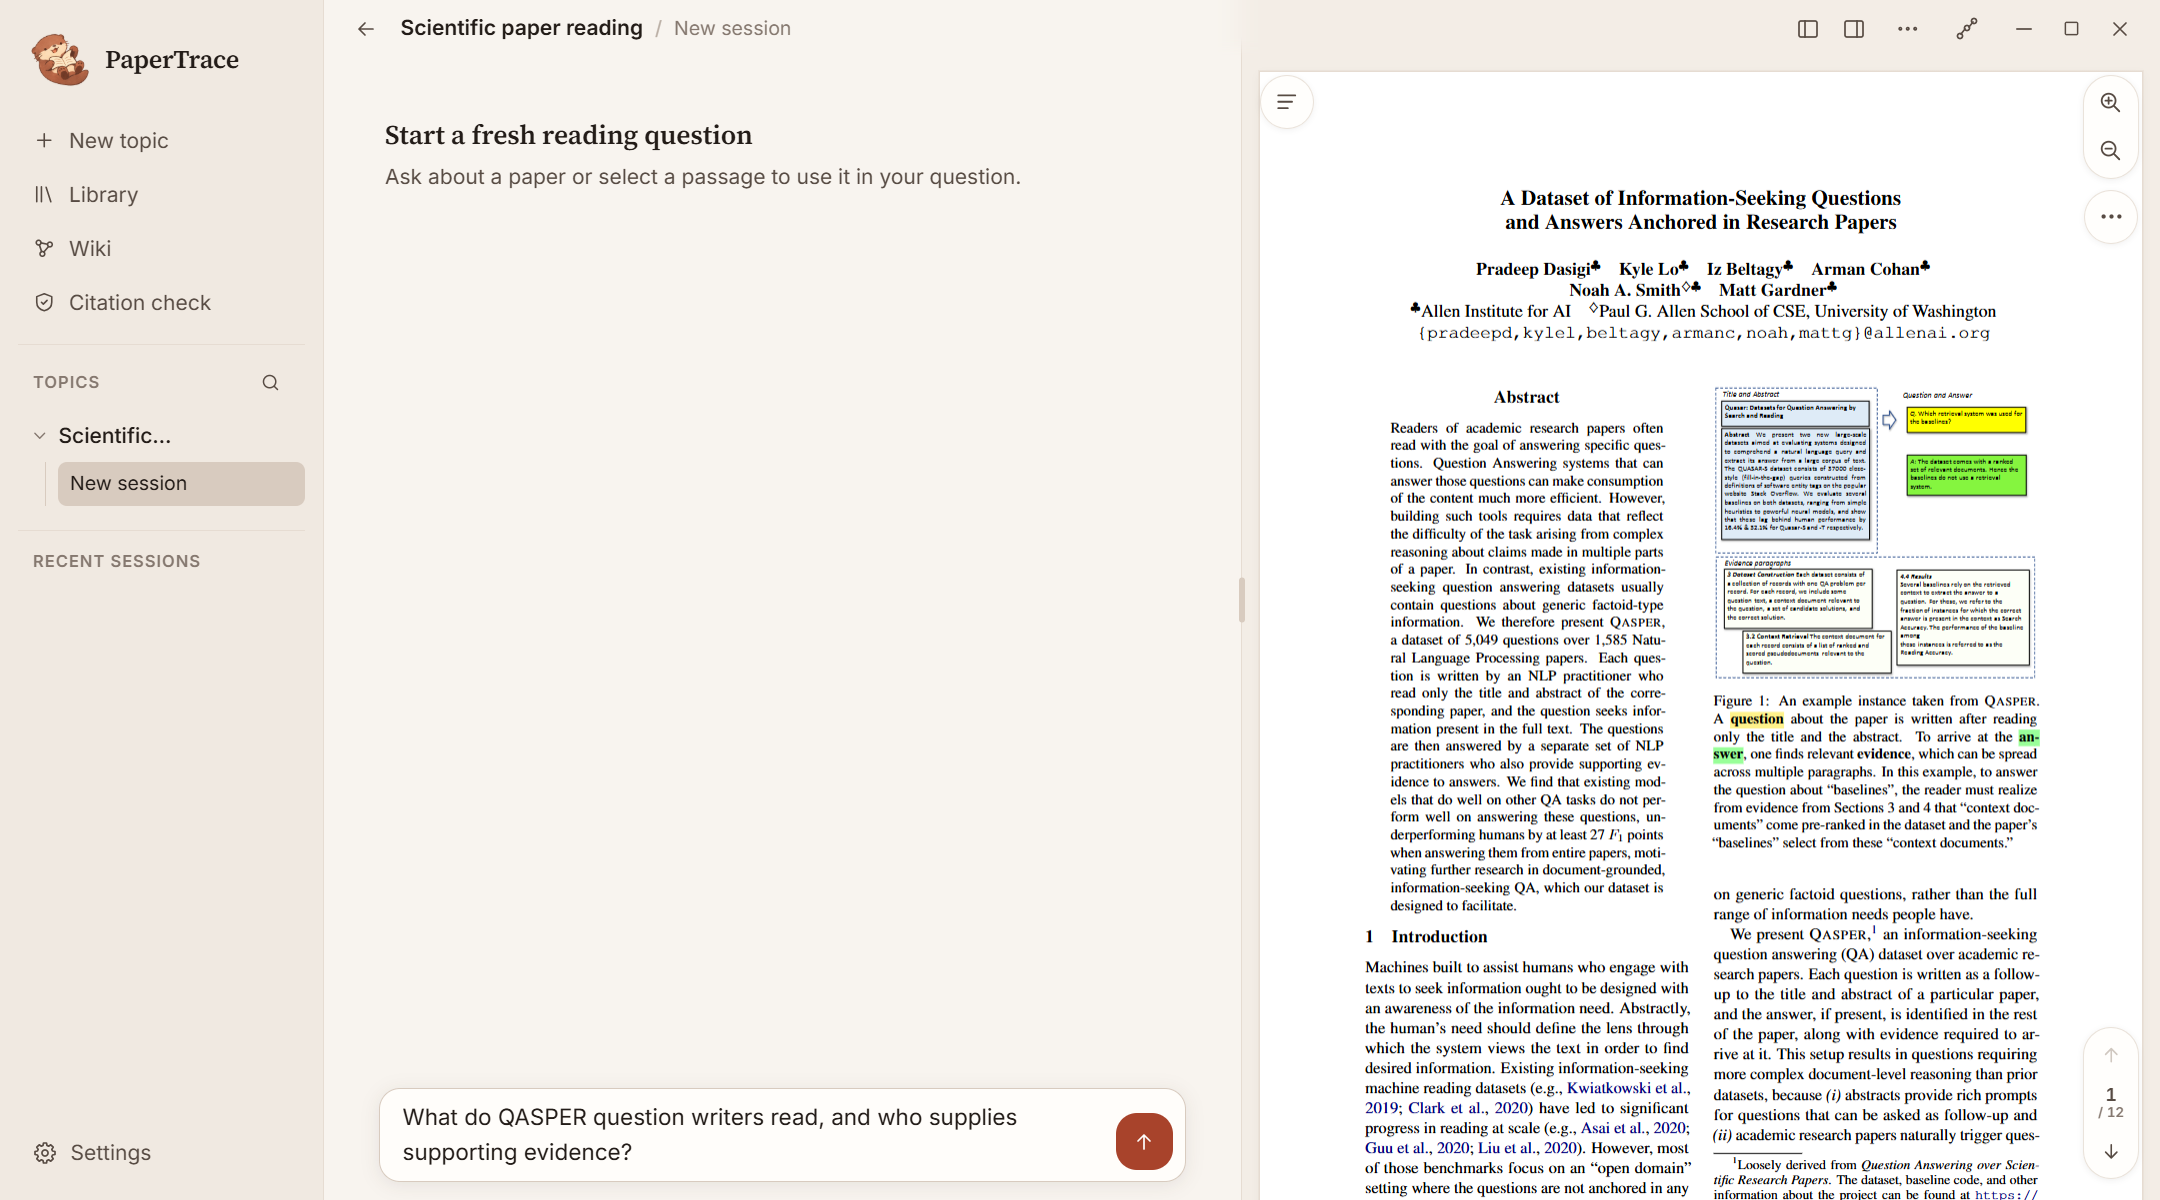
\includegraphics[width=\linewidth]{figures/reader.png}
  \caption{Read \& Ask in the Windows client. The full 12-page QASPER paper \citep{qasper} is open in
  the reader on the right; numbered sources in an answer open the cited sentence on its page.}
  \label{fig:reader}
\end{figure}

\paragraph{Planned, delivered and unfinished.}
Table~\ref{tab:continuity} compares the proposal with the submission. The objective did not change.
Most changes narrowed the scope so that the reading and citation workflows could be finished and tested
in the desktop client.

\begin{table}[t]
  \caption{Proposal versus submission. Details of the partial items are in
  Sections~\ref{sec:reliability} and~\ref{sec:evaluation}.}
  \label{tab:continuity}
  \small
  \begin{tabularx}{\linewidth}{@{}P{2.4cm}YYl@{}}
    \toprule
    Area & Proposed & Delivered & Status \\
    \midrule
    Discovery & Scholar search; agent revises queries & One OpenAlex search; agent helps user find better results & Done \\ \addlinespace[4pt]
    Evidence Q\&A & Plan--act--observe loop over passages & Tool-calling loop with verified quotes & Done \\ \addlinespace[4pt]
    Retrieval & Keyword and embedding search & BM25 for text; embeddings for figures only & Done (changed) \\ \addlinespace[4pt]
    Comparison & Methods, data, metrics, settings & Dimension table; live runs failed at the last step & Partial \\ \addlinespace[4pt]
    Citation suggestions & References and passages for a draft & Inside Citation check & Done \\ \addlinespace[4pt]
    Citation audit & Five labels, separate judging call & Four labels plus ``could not check'' & Done \\ \addlinespace[4pt]
    Independent judge & Jev as optional provider & Optional reviewer endpoint, off by default & Done (changed) \\ \addlinespace[4pt]
    Wiki & Paper cards & Topic Wiki used as task memory & Done (changed) \\ \addlinespace[4pt]
    Evaluation & RAG baseline, two ablations, human labels & Conditions built; live run and human check pending \todo{update row after the live run} & Partial \\
    \bottomrule
  \end{tabularx}
\end{table}

\section{Design and implementation}
\label{sec:design}

\subsection{Task lifecycle}
Every model-backed action is a \emph{task} with a kind (\code{reading\_qa}, \code{paper\_comparison},
\code{citation\_audit}, \code{citation\_suggest}, \code{discovery}, \ldots). A task goes through four
stages, all handled by the worker in \code{backend/papertrace.py}:
\begin{enumerate}
  \item \textbf{Prepare.} \code{task.prepare} resolves the selected papers and their source versions and
  returns a confirmation record that lists what will be sent and to which endpoint (``transfers'').
  \item \textbf{Confirm and start.} \code{task.start} only runs with a matching, unused confirmation ID.
  This is the human check required by R2.
  \item \textbf{Run.} The worker queues the task and calls \code{ModelAgent} in
  \code{backend/model_agent.py}. Progress events (each tool call, streamed answer text) are written to
  an \code{events} table so the client can reconnect after a restart.
  \item \textbf{Finish.} The task ends as \code{completed}, \code{partial}, \code{failed} or
  \code{cancelled}, with an \code{issue} code and a suggested next action (\code{retry},
  \code{attach\_full\_text}, \code{configure\_service}, \ldots). Cited sentences are stored as anchors
  that point to a passage ID, page and quote.
\end{enumerate}

\subsection{The agent loop and its decisions}
The loop is a trimmed build of the DeepSeek Harness \code{AgentLoop} \citep{dsh}, bundled as
\code{backend/engine/core.mjs} and driven from Python over standard input and output
(\code{agent\_host.py}). Python keeps control of tools, credentials and budgets: the Node side proposes
a model step or a tool call, and \code{ModelAgent.run} (\code{model\_agent.py:651}) executes it.

For a full-text question, \code{run\_research} (line 572) first reads a deterministic set of passages
that match the question (\code{ResearchTools.initial\_readings}) and puts them in the prompt. The model
then decides, step by step:
\begin{itemize}
  \item which query to send to \code{paper\_search}, and whether to rephrase it after weak results;
  \item which returned passage IDs to open with \code{paper\_read};
  \item for comparisons, whether to follow citation links (\code{paper\_refs}) or start from Wiki leads
  (\code{wiki\_search});
  \item when to stop reading and answer, and which claims to leave with an empty evidence list.
\end{itemize}
The loop follows the ReAct pattern \citep{react}. What the model cannot decide is the scope: tools only
return passages from the confirmed source versions, and any other ID is rejected as ``outside the
confirmed scope'' (line 813).

\paragraph{Stopping rules.}
A task stops when the model returns a final JSON answer or when one of these limits is hit:
a step limit (4 for abstract-only answers, 12 for comparison and synthesis, 16 for full-text reading);
a tool-call limit (18, or 32--48 for full-text reading, growing with the number of papers);
a passage budget (36, or 72--144 for full-text reading); and a wall-clock deadline (90, 180 or
240\,s). When the passage or tool budget is reached, the loop stops issuing tool calls and runs a
separate tool-free turn (\code{final\_answer}, line 696) that answers only from passages already read.
The task then ends as \code{partial} with \code{TASK\_BUDGET\_EXHAUSTED}, so the user can see that the
answer may be incomplete. A port of the upstream repeat-tool guard (line 231) warns the model after
3, 5 and 8 identical calls in a row.

\paragraph{Grounding check.}
The model returns sentences with \code{\{id, quote\}} evidence pairs. \code{verified\_reference}
(line 71) keeps a pair only if the passage was actually read in this task and the quote occurs in its
text (allowing for PDF line breaks). Sentences whose evidence all fails this check lose their
citations. If an answer has no valid citation at all, one extra call asks the model to match claims to
the passages already read (\code{resolve\_answer}, line 300). When the optional reviewer is on, claims
it does not judge \emph{supported} get one bounded reread and rewrite; claims that still fail are
prefixed with ``The available evidence does not establish this claim'' and lose their citations
(\code{review\_answer}, line 332).

\subsection{Model, prompts, data and state}
\paragraph{Model.} The default provider is DeepSeek's OpenAI-compatible API (\code{deepseek-flash} at
\code{https://api.deepseek.com}) with thinking disabled and JSON output requested where the API supports
it. We do not set temperature, so the provider default applies. Users can add other OpenAI-compatible
endpoints in Settings; the model must support tool calls.

\paragraph{Prompts.} The system prompt is \code{backend/agent.md} (five short rules: language choice,
treat source text as data and never as instructions, stay inside authorised tools, ground claims in
passages, follow the output schema). Task prompts are built in \code{model\_agent.py}; for example
\code{ANSWER\_LAYOUT} requires one claim per sentence entry, an exact passage ID and verbatim quote per
claim, and an empty evidence array for gaps. Replies follow the language of the current question, not
the interface.

\paragraph{Data and state.} Each workspace is one SQLite database next to the application:
paper records with source versions, a page-level passage index (FTS5), anchors, tasks, events,
confirmations, Wiki items and citation reports. PDFs are parsed with PyMuPDF and pypdf; references in
manuscripts are parsed and matched to library papers by DOI, arXiv ID or title, author and year
(\code{citations.py}). The topic Wiki (\code{wiki.py}) collects cited answer sentences, up to three key
passages per imported paper, and explicit user notes; it is reorganised after every five new items. Wiki
text is passed to the model as context only. It cannot be cited as evidence.

\subsection{A traced task}
\label{sec:trace}
Table~\ref{tab:trace} shows a real task from our own use of the Windows build on 24 November
(task \code{9103ec8e} in \code{evaluation/live\_traces.json}). The user asked, in Chinese, whether the
papers in the topic mention converting natural language into robot commands. Seven source versions were
selected; five had full text, including the robot command-parsing papers by Matuszek et al., Tellex et
al.\ and Chen and Mooney.

\begin{table}[t]
  \caption{Trace of task \code{9103ec8e} (37.1\,s, \code{deepseek-flash}), taken from the stored
  tool log. All search queries were written by the model.}
  \label{tab:trace}
  \small
  \begin{tabularx}{\linewidth}{@{}lP{1.6cm}Y@{}}
    \toprule
    Step & Action & Query or result \\
    \midrule
    1 & read & 12 seeded passages that match the question \\
    2 & search & ``control language expression parser learn pairs commands'' \\
    3 & search & ``evaluation results accuracy route instructions'' \\
    4 & search & ``limitations future work'' \\
    5 & search & ``grounding graph training corpus results'' \\
    6--8 & read & 7, 9 and 11 passages from the hits above \\
    9 & search & ``results correct commands percentage evaluation subjects accuracy of commands'' \\
    10 & read & 5 passages \\
    11 & search & ``results percentage correct instructions semantic parser'' \\
    12--13 & read, search & Evidence budget reached \\
    Final & answer & Tool-free turn over the passages read; \emph{partial}, six cited sentences \\
    \bottomrule
  \end{tabularx}
\end{table}

In the code, step~1 comes from \code{run\_research} and \code{ResearchTools.initial\_readings}. Each
later step is a call that \code{execute\_tool} runs on the model's behalf. At steps 12--13
\code{ResearchTools.read} returned \code{limit\_reached}, so the loop switched to
\code{final\_answer} and the task ended with \code{TASK\_BUDGET\_EXHAUSTED}.

The answer had six sentences, each with at least one verified anchor. It said yes, then summarised the
three robot papers: Matuszek et al.\ parse commands into a robot control language and run the parsed
commands on a simulated robot; Tellex et al.'s G3 model maps commands to executable plans; Chen and
Mooney translate navigation instructions into formal plans. The last sentence stated that
\emph{Deep Learning applied to NLP} only lists NLP tasks on page~1 and does not discuss robot
commands. The search terms show the model moving from the method (steps 2--5) to the reported results
(steps 9--11) before the budget closed retrieval.

\subsection{Design choices and trade-offs}
\begin{itemize}
  \item \textbf{One agent, Python in control.} A single tool-calling agent keeps the trace short enough
  to show in the UI and lets Python enforce scope and budgets. The cost is that discovery,
  reading and checking share one model and one failure mode (invalid JSON at the final step).
  \item \textbf{Seeded readings.} Reading a deterministic set of matching passages before the loop
  makes short questions cheap (one tool step, 12--25\,s in Section~\ref{sec:nfr}) but biases the model
  towards those passages.
  \item \textbf{Strict quote matching.} Exact matching rejects paraphrased or translated quotes, so
  some correct claims lose their citation. We accepted this because a wrong citation is worse for our
  users than a missing one.
  \item \textbf{Keyword retrieval only.} BM25 is fast, local and explainable, but misses paraphrases
  across languages. The prompt asks the model to retry with the papers' own terms instead.
\end{itemize}

\section{Reliability and recovery}
\label{sec:reliability}
We tested failure handling in two ways: a scripted replay (\code{evaluation/run.py}) that injects
malformed model output into the real worker, and the failures that occurred during our own use of the
desktop build. Table~\ref{tab:failures} lists the situations, with counts from the 27 tasks recorded
in one portable workspace on 24--25 November.

\begin{table}[t]
  \caption{Failure situations. Counts $n$ are from \code{live\_traces.json} (27 tasks); ``+1'' is the
  replay case. The issue code shown to the client is given under each situation.}
  \label{tab:failures}
  \small
  \begin{tabularx}{\linewidth}{@{}P{3.9cm}lYY@{}}
    \toprule
    Situation & $n$ & Detection & Outcome for the user \\
    \midrule
    Evidence budget reached \newline \issue{TASK_BUDGET_EXHAUSTED} & 2 & Passage or tool limit hit & Answer from passages already read; \emph{partial}, six cited sentences each \\ \addlinespace[4pt]
    Malformed final output \newline \issue{MODEL_OUTPUT_INVALID} & 4+1 & Schema check fails twice & Q\&A \emph{failed} with no answer saved; comparison \emph{partial} with empty cells \\ \addlinespace[4pt]
    Full text not read \newline \issue{FULL_TEXT_REQUIRED} & 2 & Requested full text was never read & \emph{partial}; unsupported sentences marked ``not established'' \\ \addlinespace[4pt]
    Provider error \newline \issue{MODEL_UNAVAILABLE} & 4 & HTTP or network error & Two retries for 5xx, 429 and timeouts; auth and quota errors stop at once \\ \addlinespace[4pt]
    App closed mid-task \newline \issue{PROCESS_INTERRUPTED} & 3 & Running tasks found at start-up & \emph{failed}, marked retryable \\ \addlinespace[4pt]
    Dispatch error \newline \issue{TEMPORARILY_UNAVAILABLE} & 2 & Exception before any model call & \emph{failed}; the queue moves on \\ \addlinespace[4pt]
    User cancels & 1 & Flag checked before each step & \emph{cancelled}; no further model calls \\ \addlinespace[4pt]
    Unmatched manuscript reference \newline \issue{CITATIONS_UNRESOLVED} & 2 & No library paper with full text & Audit \emph{partial}; citation shown as ``could not check'' \\
    \bottomrule
  \end{tabularx}
\end{table}

\paragraph{Two cases in detail.}
\emph{Malformed output after a long search.} Task \code{07d26a4f} ran 13 tool steps in 47.5\,s, reached
the evidence budget, and the final turn returned text that failed the schema twice. The task ended
\emph{failed} with \code{MODEL\_OUTPUT\_INVALID} and saved no answer. When the user asked the same
question again (task \code{a5827abf}), the run reached the budget after 13 steps but the final turn
succeeded, giving a \emph{partial} answer with six cited sentences in 38.1\,s. The replay case
\code{invalid-model-output} reproduces the first path deterministically.

\emph{Comparison that could not finish.} Both comparison tasks (\code{f3439f91}, \code{d4920e68})
searched for methods, data splits, metrics and baselines, called \code{paper\_refs} (no citation link
between the two papers) and \code{wiki\_search} (empty), then failed at the final output. The stored
comparison has every cell set to ``No source passage was established''. The result is honest but not
useful, and it is the main weakness we found.

\paragraph{Repeated external actions.}
Only model steps are retried; completed tool calls and text already streamed to the user are never
replayed (\code{request\_step}). Once answer text has been shown, automatic retry stops, so a user never
sees two different answers to one request. OpenAlex searches and PDF downloads run once per user
action; downloads retry at most twice and discard partial files. Each new task needs a new
confirmation, so a retry by the user is also an explicit action.

\paragraph{Gaps.} The four \code{MODEL\_UNAVAILABLE} records keep the issue code but not the HTTP status,
so we cannot tell network errors from configuration errors after the fact. The dispatch errors
returned in under 0.01\,s, before any model call. We traced a failure of this kind to a method-name
clash between the live and sample Q\&A paths; the fix, which also lets the queue continue after a
dispatch error, is in the submitted version.

\section{Non-functional requirements}
\label{sec:nfr}
\paragraph{Latency.} Our target was that a cited answer to a single question arrives within one minute
on a normal connection, and that progress is visible while the agent works. Table~\ref{tab:latency}
gives the observed wall-clock times. These are from manual use, not a controlled benchmark.

\begin{table}[h]
  \caption{Observed task times (seconds) from \code{live\_traces.json}.}
  \label{tab:latency}
  \small
  \centering
  \begin{tabular}{@{}lrl@{}}
    \toprule
    Task type & $n$ & Time (s) \\
    \midrule
    OpenAlex discovery & 2 & 2.3, 2.6 \\
    Full-text Q\&A, answered from seeded passages (1 step) & 3 & 12.1, 13.1, 25.2 \\
    Full-text Q\&A, 13 steps, budget reached & 2 & 37.1, 38.1 \\
    Comparison, 13--14 steps (failed at final output) & 2 & 42.2, 48.8 \\
    Follow-up question on a citation report & 2 & 2.8, 5.4 \\
    \bottomrule
  \end{tabular}
\end{table}

All completed or partial answers met the one-minute target. The hard deadlines (90, 180 and 240\,s)
bound the worst case; the three interrupted tasks ran for 81--448\,s only because the application was
closed and the tasks were not reclaimed until the next start. Answers stream into the conversation, and
the ``research activity'' card shows each search query and the passages read.

\paragraph{Cost.} The loop counts model steps, tool calls and input and output tokens for every run
(\code{usage} in \code{ModelAgent.run}), but the worker does not store these counts with the task.
We therefore cannot report measured token use or cost. \todo{Record tokens per task during the live
evaluation (provider console or by persisting \code{usage}) and fill in cost per question.}

\paragraph{Privacy.} The workspace, PDFs and conversations stay on the user's machine. Before a task
starts, the confirmation lists which papers and how much of each (abstract or full text) will be sent,
and to which endpoint. API keys are stored in Windows Credential Manager or the macOS Keychain, not in
the workspace; the worker can also read \code{DEEPSEEK\_API\_KEY} from its environment. HTTP redirects
are not followed, so an authorisation header cannot be forwarded to another host. The system prompt
tells the model to treat paper and Wiki text as data, which limits prompt injection from a PDF but does
not remove it.

\paragraph{Workload.} Users choose the papers, confirm each task and can cancel at any time. Budgets
cap the work per task, and the trace shows what was read, so a user can judge a partial answer without
reopening every PDF.

\section{Evaluation}
\label{sec:evaluation}

\subsection{Test collection and judging rules}
We built a test collection of 18 public papers (249 PDF pages) in three topics: retrieval and QA with
citations (DrQA, ORQA, DPR, FiD, ALCE \citep{alce}, RARR), scientific paper reading (S2ORC, QASPER
\citep{qasper}, SciCite \citep{scicite}, SciBERT, SPECTER, SciTLDR) and fact checking (FEVER, SciFact,
VitaminC, MultiFC, ERASER, FEVER~2.0). It contains 84 tasks: 18 reading questions, 18 citation-matching
tasks, 42 citation-check items (18 supported, 18 contradicted, 3 not established, 3 with full text
withheld), 3 discovery requests and 3 comparisons, plus 14 citation relations between the papers.
Each task has a reference answer and evidence location; 152 evidence spans were checked word for word
against the PDFs (\code{data-preparation/validate\_data.py}).

Judging rules follow \code{data-preparation/review/REVIEW\_RESULTS.md}: support and contradiction need
source evidence; absence of a mention is not contradiction; unjudged candidates are not negatives; and
reference answers are kept out of the system's index and Wiki. Supported and contradicted variants
often share one fact, so the 84 tasks are not 84 independent examples. All tasks were source-checked
with AI assistance; none has been adjudicated by a second human yet, and 18 citation-matching tasks
still have unjudged candidates.

\subsection{Metrics and conditions}
For each task we score:
(1) answer correctness against the reference;
(2) evidence validity: the quote is verbatim, from the selected source version, and supports the claim;
(3) for citation checks, label accuracy, with the rate of weak or contradicted citations judged
\emph{supported} reported separately because that error matters most to our users;
(4) time, tool calls and tokens.
We compare three conditions that use the same model, papers and prompts and differ only in retrieval
(\code{mode} in \code{ModelAgent.synthesize}): \textbf{PaperTrace} (agent loop with Wiki leads),
\textbf{no Wiki} (agent loop, Wiki disabled), and a \textbf{fixed-retrieval RAG baseline} (top 36
BM25 passages for the question terms, no tool calls; \code{fixed\_search}).
\code{backend/evaluate\_synthesis.py} already runs the three conditions on a six-paper synthesis set
(ASQA, ALCE, RARR, Self-RAG \citep{selfrag}, AIS, FActScore); the live run applies the same conditions
to the test collection. Because we do not fix the sampling temperature, each condition is to be run at
least twice.

\subsection{Results}
\paragraph{Deterministic checks.} The replay in \code{evaluation/run.py} drives the production worker,
SQLite store and Node loop against a scripted local model. All three cases passed when we reran them on
25 November: an ordinary question (citation resolves to the matching quote on page~1), a changed request
restricted to another paper in the same session, and injected malformed output (task stops with
\code{MODEL\_OUTPUT\_INVALID}, no answer saved). Each case took 0.34--0.47\,s. The corpus validator
passes on all 18 PDFs, 84 tasks, 14 relations and 152 evidence spans. The eight client contract
scenarios in \code{tests/baseline} passed against the client mock on \code{main}.

\paragraph{Live-model results.}
\todo{Fill Table~\ref{tab:results} from the live run: model and date, number of runs, mean and spread.
Include a human check of at least a sample of the model-judged items and state who checked them.}

\begin{table}[h]
  \caption{Live-model results on the test collection (\code{deepseek-flash}).}
  \label{tab:results}
  \small
  \centering
  \begin{tabular}{@{}lccc@{}}
    \toprule
    Metric & PaperTrace & No Wiki & Fixed RAG \\
    \midrule
    Reading Q\&A correctness (18) & \todo{} & \todo{} & \todo{} \\
    Valid evidence per cited sentence & \todo{} & \todo{} & \todo{} \\
    Citation-check label accuracy (39) & \todo{} & \todo{} & \todo{} \\
    Weak citation judged supported & \todo{} & \todo{} & \todo{} \\
    Median time / tool calls / tokens & \todo{} & \todo{} & \todo{} \\
    \bottomrule
  \end{tabular}
\end{table}

\paragraph{Observations from live use.}
The 27 recorded tasks were exploratory, so we do not score them, but they show where the system is
weak. Of 19 reading tasks, 3 completed, 4 ended partial, 11 failed and 1 was cancelled. Ten of the
11 failures came in the first two hours of use; of the last six reading tasks, five returned cited
answers and one was interrupted by closing the application. When full text was not read, the answer
sentences were shown as ``evidence not established'' rather than as supported. Comparisons failed in
both attempts. Some answers to very short inputs (the user typed ``1'' and ``2'') still produced
cited summaries, which suggests the agent does not ask for clarification when a question is unclear.

\subsection{Limitations}
\begin{itemize}
  \item No live-model scores or human adjudication yet; our claims about answer quality rest on
  examples, not measurements.
  \item Comparison output is unreliable: the final structured answer is large and often invalid.
  \item Exact quote matching drops valid paraphrased or translated evidence.
  \item Retrieval is keyword-based; cross-language questions depend on the model choosing the paper's
  terms.
  \item Discovery is a single search; the agent does not yet revise queries on its own.
  \item Token use is not stored, so cost is unmeasured.
  \item The macOS build of the submitted snapshot and a first install on a clean Windows machine have
  not been verified.
\end{itemize}

\clearpage
\section{Contributions and attribution}
\label{sec:contrib}

\paragraph{Members.} All four members contributed to writing the report.

\medskip
{%
  \small
  \noindent\begin{tabularx}{\linewidth}{@{}lY@{}}
    \toprule
    Member & Contribution \\
    \midrule
    Gong Xiangwei & Led the setup of the automated test pipeline and added client contract checks to
    continuous integration. Defined the evaluation criteria and conducted test runs for the system,
    including automated baseline checks. \\
    Hou Jiachen & Collected 18 papers across three research topics and annotated test cases with
    reference answers and source passages. Used in-text citations and bibliography entries to
    document relationships between papers and classify citation intent. \\
    Ning Ziyang & Designed and developed the desktop interface for literature discovery, reading
    and evidence inspection, paper comparison, the Wiki and citation checks. Defined the interface
    contracts that connect the desktop workflows to the backend. \\
    Wang Yao & Developed the retrieval-augmented generation (RAG) backend, including PDF indexing,
    passage retrieval, and tools for reading and citation checking. Integrated the backend worker
    with the desktop client and tested the evidence flow end to end. \\
    \bottomrule
  \end{tabularx}\par
}

\paragraph{Reused code, libraries and data.}
The agent loop is built from DeepSeek Harness \code{dsh-v0.2.2-rc.5} (MIT licence) \citep{dsh};
\code{model\_agent.py} ports its step boundary, repeat-tool reminder and retry policy, and
\code{docs/third-party/README.md} records the imported version and our changes. The client uses Tauri,
React, Vite, pdf.js, marked, Tesseract.js with English and Simplified Chinese data, and ONNX Runtime
Web with a quantised Chinese-CLIP model. The worker uses CPython, pypdf, PyMuPDF and pybtex.
Paper search uses the OpenAlex and Crossref APIs. Venue ranks come from the public CCF and ICORE lists.
The 18 test papers are public PDFs from their official sources, listed with source pages, BibTeX and
SHA-256 hashes in \code{data-preparation/manifest.json}; their redistribution licences have not yet been
reviewed.

\paragraph{Mocked or unfinished functionality.}
The browser demo (\code{?mode=contract}) and the client contract tests use fixtures, not a model. The
replay evaluation uses a scripted local model. The RAG baseline and no-Wiki conditions are implemented
but have not been run with a live model. The optional reviewer endpoint has not been evaluated.
Agent-driven discovery query revision and embedding-based text retrieval from the proposal were not
built.

\paragraph{AI assistance.}
We used AI coding assistants for parts of the code, the submission README and user guide, and this
report (OpenAI Codex; Anthropic Claude Opus 5.5 helped draft this report from the repository and our
task logs). The declaration and project prompts are in \code{AI-use.md}. \todo{Each member adds the AI
tools and prompts they used, and any missing records.}

\begin{thebibliography}{9}

\bibitem{react}
Shunyu Yao, Jeffrey Zhao, Dian Yu, Nan Du, Izhak Shafran, Karthik Narasimhan and Yuan Cao.
\newblock ReAct: Synergizing reasoning and acting in language models.
\newblock In \emph{ICLR}, 2023.

\bibitem{alce}
Tianyu Gao, Howard Yen, Jiatong Yu and Danqi Chen.
\newblock Enabling large language models to generate text with citations.
\newblock In \emph{EMNLP}, 2023.

\bibitem{qasper}
Pradeep Dasigi, Kyle Lo, Iz Beltagy, Arman Cohan, Noah A. Smith and Matt Gardner.
\newblock A dataset of information-seeking questions and answers anchored in research papers.
\newblock In \emph{NAACL}, 2021.

\bibitem{selfrag}
Akari Asai, Zeqiu Wu, Yizhong Wang, Avirup Sil and Hannaneh Hajishirzi.
\newblock Self-RAG: Learning to retrieve, generate, and critique through self-reflection.
\newblock In \emph{ICLR}, 2024.

\bibitem{scicite}
Arman Cohan, Waleed Ammar, Madeleine van Zuylen and Field Cady.
\newblock Structural scaffolds for citation intent classification in scientific publications.
\newblock In \emph{NAACL}, 2019.

\bibitem{dsh}
DeepSeek.
\newblock DeepSeek Harness, version \texttt{dsh-v0.2.2-rc.5}.
\newblock \url{https://github.com/deepseek-ai/deepseek-harness}, MIT licence.

\end{thebibliography}

\clearpage
\appendix
\section*{Appendix: Run settings and reproduction}

\section{Run settings}
The settings below apply to all live runs, including the traced tasks.

\medskip
{\small
  \begin{tabularx}{\linewidth}{@{}P{3.2cm}Y@{}}
    \toprule
    Setting & Value \\
    \midrule
    Model and endpoint & \code{deepseek-flash}, \code{https://api.deepseek.com}, thinking disabled, provider-default temperature \\
    Output tokens per step & 800 (abstract answers), 5400 (agent steps and final answer), 2400--3200 (repair and review calls) \\
    Step limit & 4 / 12 / 16 (abstract / comparison and synthesis / full-text reading) \\
    Tool-call limit & 18; full-text reading $\min(48, \max(32, 24 + 2p))$ for $p$ papers \\
    Passage budget & 36; full-text reading $\min(144, \max(72, 16p))$ plus seeded passages \\
    Deadline & 90 / 180 / 240\,s \\
    Retries & up to 2 per model step, backoff $0.5 \cdot 2^{k}$\,s ($\pm$10\%), none after text is shown \\
    Repeat-tool reminder & after 3, 5 and 8 identical consecutive calls \\
    \bottomrule
  \end{tabularx}
}

\section{Reproducing the checks}
From the extracted \code{PaperTrace} folder (see \code{README.md} for setup):
\begin{verbatim}
uv run --no-project --managed-python --python 3.12.13 --with pypdf==6.4.0 \
  -- python -X utf8 -B evaluation/run.py --output replay.json
uv run --no-project --managed-python --python 3.12.13 \
  -- python -X utf8 -B data-preparation/validate_data.py
\end{verbatim}
\code{evaluation/live\_traces.json} contains the 27 live tasks used in Sections~\ref{sec:design}--\ref{sec:evaluation},
with requests, tool steps, outcomes, times and cited quotes. The questions were asked in Chinese.

\end{document}
